\begin{figure}[t]
\begin{center}
\begin{small}
\begin{sc}
\begin{tabular}{c@{\hskip2pt}c@{\hskip2pt}c@{\hskip2pt}c}
Input&Ours&GlAtEx&AttSeg\\
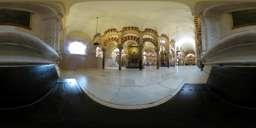
\includegraphics[width=\smallimg]{fig/sun360/1/gt.jpg}&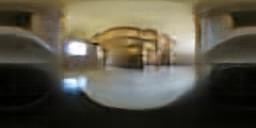
\includegraphics[width=\smallimg]{fig/sun360/1/ours.jpg}&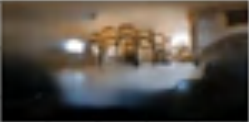
\includegraphics[width=\smallimg]{fig/sun360/1/glatex.png}&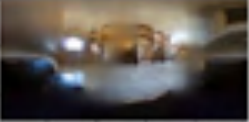
\includegraphics[width=\smallimg]{fig/sun360/1/atseg.png}\\

\includegraphics[width=\smallimg]{fig/sun360/2/gt.jpg}&
\includegraphics[width=\smallimg]{fig/sun360/2/ours.jpg}&
\includegraphics[width=\smallimg]{fig/sun360/2/glatex.png}&
\includegraphics[width=\smallimg]{fig/sun360/2/atseg.png}\\

\includegraphics[width=\smallimg]{fig/sun360/3/gt.jpg}&
\includegraphics[width=\smallimg]{fig/sun360/3/ours.jpg}&
\includegraphics[width=\smallimg]{fig/sun360/3/glatex.png}&
\includegraphics[width=\smallimg]{fig/sun360/3/atseg.png}\\

\includegraphics[width=\smallimg]{fig/sun360/5/gt.jpg}&
\includegraphics[width=\smallimg]{fig/sun360/5/ours.jpg}&
\includegraphics[width=\smallimg]{fig/sun360/5/glatex.png}&
\includegraphics[width=\smallimg]{fig/sun360/5/atseg.png}\\
\end{tabular}
\end{sc}
\end{small}
\end{center}
\vskip -0.1in
\caption{\textbf{Reconstruction quality for SUN360:} Reconstruction results of our method compared with AttSeg~\protect\cite{seifi2020segment} and GlAtEx~\protect\cite{seifi2021glimpse} on the SUN360 dataset. Reconstructions done with our method are visibly better than the competition.}
\label{fig:qualiative-retinal}
\end{figure}